\section{Geometrie}
\subsection{Planimetrie}
\subsubsection{Strahlensätze}
%TODO picture
\paragraph{1.}
\begin{align*}
    \overline{SA_1} : \overline{SB_1} = \overline{A_1A_2} : \overline{B_1B_2} \\
    \overline{SA_1} : \overline{SA_1} = \overline{SB_1} : \overline{SB_2} \\
\end{align*}
Entsprechende Abschnitte auf den Strahlen stehen im gleichen Verhältnis

\paragraph{2.}
\begin{align*}
    \overline{CB} : \overline{C_1B_1}: \overline{C_2B_2}    &= \overline{SC} : \overline{SC_1} : \overline{SC_2}  \\
                                                            &= \overline{SB} : \overline{SB_1} : \overline{SB_2}  \\
\end{align*}
\begin{align*}
    \overline{AB} : \overline{A_1B_1}: \overline{A_2B_2}    &= \overline{SA} : \overline{SA_1} : \overline{SA_2}  \\
                                                            &= \overline{SB} : \overline{SB_1} : \overline{SB_2}  \\
\end{align*}
Entsprechende Abschnitte auf den Parallelen stehen im gleichen Verhältnis wie die zugehörigen, vom Scheitel aus zu messenden Abschnitte auf den Strahlen.

\paragraph{3.}
\begin{align*}
    \overline{AB} : \overline{BC} = \overline{A_1B_1} : \overline{B_1C_1} = \overline{A_2B_2} : \overline{B_2C_2} \\
\end{align*}
Entsprechende Abschnitte auf den Parallelen stehen im gleichen Verhältnis.

\subsubsection{Satz des Pythagoras}
%TODO picture
\begin{align*}
    a^2+b^2=c^2
\end{align*}

\subsubsection{Höhensatz des Euklid}
%TODO picture
\begin{align*}
    h^2=p \cdot q
\end{align*}


%\begin{figure}[htb]
%\begin{center}
%	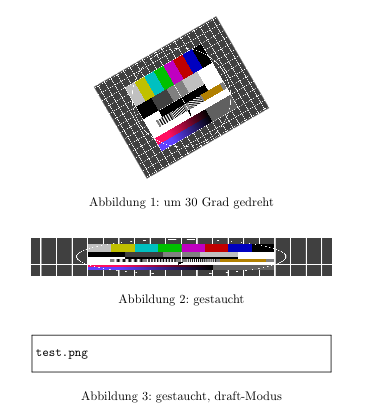
\includegraphics[height=1in,width=1in,angle=-90]{sections/08_Geometrie/pythagoras.standalone.pdf}
%\caption{This is a figure.}
%\end{center}
%\end{figure}

%\begin{figure}
%    \centering
%    \subfloat{
%	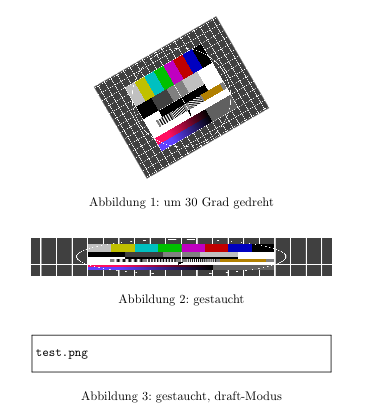
\includegraphics[height=2in,width=2in,angle=-90]{sections/08_Geometrie/pythagoras.standalone.pdf} 
%   }\hfill
%   \subfloat{
%      \begin{minipage}[t]{120mm}
%   	$A = \frac{d^2 \cdot \pi}{4}$ \\
%	$U = d \cdot \pi  $
%      \end{minipage}
%    }
%  \caption{Abbildungsname}
%  \label{fig:decision-tree}
%\end{figure}

\subsubsection{Kathetensatz}
%TODO picture
\begin{align*}
    a^2=c \cdot p \\
    b^2=c \cdot q \\
\end{align*}

\subsubsection{Trapez}
%TODO picture
\begin{align*}
    A &= \frac{a+b}{2} \cdot h = m \cdot h \\
    m &= \frac{a+b}{2}
\end{align*}

\subsubsection{Kreis}
%TODO picture
\begin{align*}
    A &= \frac{d^2 \cdot \pi}{4} \\
    U &= d \cdot \pi \\
\end{align*}

\subsubsection{Kreisausschnitt}
%TODO picture
\begin{align*}
    A &= \frac{d^2 \cdot \pi}{4} \cdot \frac{\alpha^\circ}{360^\circ} = \frac{b \cdot r}{2} \\
    b &= \frac{d \cdot \pi \cdot \alpha^\circ }{ 360^\circ} \\
\end{align*}

\subsubsection{Ellipse}
%TODO picture
\begin{align*}
    A &= \frac{D \cdot d \cdot \pi}{4} = a \cdot b \cdot \pi \\
    U &\approx \frac{D+d}{2} \cdot \pi \\
\end{align*}


\subsection{Stereometrie}
\paragraph{Gerade Körper}
\begin{align*}
    V = A \cdot h
\end{align*}

\paragraph{Spitze Körper}
\begin{align*}
    V = \frac{1}{3} \cdot A \cdot h
\end{align*}

\paragraph{Stumpfe Körper}
\begin{align*}
    V = \frac{1}{3} \cdot h ( A_1 + \sqrt{A_1 \cdot A_2} + A_2)
\end{align*}

\paragraph{Kugel}
\begin{align*}
    V &= \frac{4}{3} \cdot \pi \cdot r^3 \\
    O &= 4 \cdot \pi \cdot r^2 \\
\end{align*}

\subsection{Trigonometrie}
\subsubsection{Winkelfunktionen im rechtwinklichen Dreieck}
%TODO picture
\begin{align*}
    \sin \alpha &= \frac{\textrm{Gegenkathete}}{\textrm{Hypotenuse}}  &= \frac{a}{c} \\
    \cos \alpha &= \frac{\textrm{Ankathete}}{\textrm{Hypotenuse}}     &= \frac{b}{c} \\
    \tan \alpha &= \frac{\textrm{Gegenkathete}}{\textrm{Ankathete}}   &= \frac{a}{b} \\
    \cot \alpha &= \frac{\textrm{Ankathete}}{\textrm{Gegenkathete}}   & = \frac{b}{a} \\
\end{align*}

\subsubsection{Winkelfunktionen im spitz- und stumpfwinklichen Dreieck}
%TODO picture
\begin{align*}
\end{align*}

\paragraph{Sinussatz}
%TODO picture
\begin{align*}
\end{align*}

\paragraph{Kosinussatz}
\begin{align*}
\end{align*}

\paragraph{Fläche eines Dreiecks}
\begin{align*}
\end{align*}


\subsection{Geniometrie}